\chapter{Learning About Oneself}

This chapter follows J. Krishnamurti's San Diego public talk of April 5, 1970, preserved in Krishnamurti Foundation Trust source material and curated here by LazyingArt LLC through Video2Book. The talk is not a mathematical lecture, and no validated blackboard screenshots remain for this chapter. The displayed formulas are therefore not recovered board equations; they are compact notation for the lecture's internal logic. We use them as a disciplined map of the inquiry, while keeping the conceptual distinctions faithful to the spoken source.

\section{The World As Contradiction}

Krishnamurti begins with the widest field: wherever one goes, in Europe, India, Australia, or America, the same human problems appear. Human beings are confused, unhappy, miserable, sorrowful, and caught in contradiction. Life appears as a battlefield, and the world is divided by nationality, language, religion, profession, ideology, and mutually opposed claims to the one right way.

The point of this opening is not a survey of world affairs. It is the pressure that makes the question of action unavoidable. The lecture gathers the disorder of human life into a simple movement:
\begin{equation}
\text{division}
\;\longrightarrow\;
\text{contradiction}
\;\longrightarrow\;
\text{conflict}
\;\longrightarrow\;
\text{violence}
\;\longrightarrow\;
\text{sorrow}.
\end{equation}
This is not a theorem and not a causal law. It is a notation for the rhythm of the opening: division appears outwardly, is found inwardly, and expresses itself as conflict and sorrow.

The important transition is that outward disorder and inward disorder are not kept apart. The world is divided into nations, sects, institutions, and opinions; the person is divided by belief, fear, ambition, anger, comparison, prejudice, and desire. The lecture will keep returning to this symmetry until the question ``what is one to do?'' becomes inseparable from the question ``how does one observe oneself?''

\section{What Is One To Do?}

Seeing all this division and misery, one asks what course of action is to be followed. Krishnamurti lets the usual answers appear one after another: left, center, right, ideology, belief, authoritarian dictum, guru, teacher, priest, organized religion, personal inclination, experience, knowledge, self-reliance, confidence, and purpose.

The first technical point in the inquiry is that these alternatives are not yet whole. They may seem opposed to one another, but each can operate as a fragment that claims authority over life. As shorthand:
\begin{equation}
\text{fragmentary action}
=
\{\text{politics},\text{belief},\text{authority},
\text{inclination},\text{experience},\text{knowledge}\}.
\end{equation}
The set notation is only a working device. It says that a political answer, a religious answer, and a personal answer may all belong to the same structure if each begins from a divided center.

\subsection{Question \& Answer}

\paragraph{Question.}
If the world is contradictory, should one follow a political direction, a religious authority, a teacher, a personal tendency, or one's own accumulated experience?

\paragraph{Answer.}
Krishnamurti does not choose among these alternatives. He asks whether there is an action that is not broken up, not contradictory, and not productive of further sorrow. The inquiry therefore changes shape:
\begin{equation}
\text{world disorder}
\;\longrightarrow\;
\text{what is one to do?}
\;\longrightarrow\;
\text{whole action}.
\end{equation}

Whole action is first approached by negation. It is not dictated by authority, not imitation, not dependency, not theory, not philosophical concept, and not an abstract ideal. It must be an actual way of living.

\begin{figure}
\centering
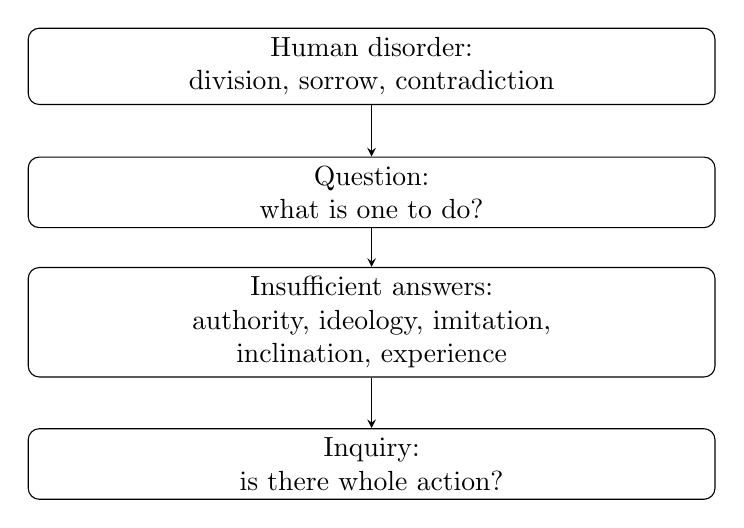
\begin{tikzpicture}[>=stealth]
\node[draw, rounded corners, text width=.70\linewidth, align=center] (a) at (0,0) {Human disorder:\\division, sorrow, contradiction};
\node[draw, rounded corners, text width=.70\linewidth, align=center] (b) at (0,-1.6) {Question:\\what is one to do?};
\node[draw, rounded corners, text width=.70\linewidth, align=center] (c) at (0,-3.25) {Insufficient answers:\\authority, ideology, imitation,\\inclination, experience};
\node[draw, rounded corners, text width=.70\linewidth, align=center] (d) at (0,-5.05) {Inquiry:\\is there whole action?};
\draw[->] (a) -- (b);
\draw[->] (b) -- (c);
\draw[->] (c) -- (d);
\end{tikzpicture}
\end{figure}

\section{Whole Action And The Speaker As Mirror}

The word ``religion'' is then used in a precise local sense. Krishnamurti does not mean belief in God, no-God, or any conceptual ideation. He means a way of life in which every action is whole, complete, and not contradictory. This is a decisive pivot: the talk moves from choosing a program to investigating the quality of action itself.

We can keep the contrast visible:
\begin{equation}
\text{fragmentary action}
\neq
\text{whole action}.
\end{equation}
Fragmentary action proceeds from division, authority, image, imitation, dependency, or accumulated knowledge. Whole action is not an occasional response in crisis. It must operate in daily life, every minute, in relationship, thought, speech, and conduct.

Before entering the detailed inquiry, Krishnamurti establishes the relation between speaker and listener. The speaker is not teaching in the ordinary informational sense. Mathematics or scientific information may be taught; here the listener is not receiving a doctrine. The words are to function as a mirror in which one's own reactions and conditioning become visible.

\begin{equation}
\text{speaker's words}
\;\longrightarrow\;
\text{listener's reactions}
\;\longrightarrow\;
\text{observation of oneself}.
\end{equation}

This matters for the whole chapter. We are not trying to collect conclusions. We are following a movement of observation. Communication, in this sense, means sharing together, understanding together, and working together.

\begin{table}
\centering
\begin{tabular}{p{.42\linewidth}p{.42\linewidth}}
\textbf{Information-learning} & \textbf{Self-learning} \\
Mathematics or scientific information may be taught. & Self-understanding cannot be handed over. \\
The teacher gives content. & The speaker functions as a mirror. \\
Knowledge is accumulated. & Reaction is observed as it arises. \\
Authority may organize the subject. & Authority would distort the inquiry. \\
\end{tabular}
\end{table}

\section{The World Is You}

After establishing this relationship, Krishnamurti returns to the question of the world. We ordinarily ask what to do about society as though society were outside us. But the talk now removes that distance. The world is made of greed, anger, ambition, competition, violence, prejudice, and antagonism; inwardly, we are that. The disorder is not merely external.

The pivot can be written as
\begin{equation}
\text{world} = \text{oneself}
\quad\Longrightarrow\quad
\text{responsibility} = \text{understanding oneself}.
\end{equation}
This is not a metaphysical identity. It is a compact notation for the lecture's claim that the world one wants to change is not separate from the human being who has made it.

\subsection{Question \& Answer}

\paragraph{Question.}
If the world is violent and confused, should one ask which party, movement, group, or reform to join?

\paragraph{Answer.}
That question still treats the world as something outside oneself. Once one sees that one's own ambition, fear, anger, prejudice, and violence are part of the world, the question has a different meaning. Responsibility is no longer primarily the selection of an outer label. It becomes the complete understanding of oneself.

So the original question has been transformed:
\begin{equation}
\text{what should I do about the world?}
\;\longrightarrow\;
\text{how do I observe myself?}
\end{equation}

\section{How To Observe}

The central refrain now appears: how do you observe? Krishnamurti first removes labels. American, Indian, British, religious, ideological, and social labels do not reach the ordinary human being underneath. Then he uses the word ``individual'' in its literal force: indivisible. By that standard, the contradictory human being is not yet an individual.

The distinction is useful:
\begin{align}
\text{individual} &:= \text{an undivided human being},\\
\text{ordinary self} &:= \text{a fragmented, contradictory movement}.
\end{align}

The difficulty sharpens. If the self is fragmented, can one fragment observe the rest? If one fragment becomes censor, examiner, analyser, or observer, what gives it authority over the other fragments? The lecture is careful here: the problem is not only professional analysis. Self-analysis may repeat the same pattern if a fragment takes charge.

\begin{figure}
\centering
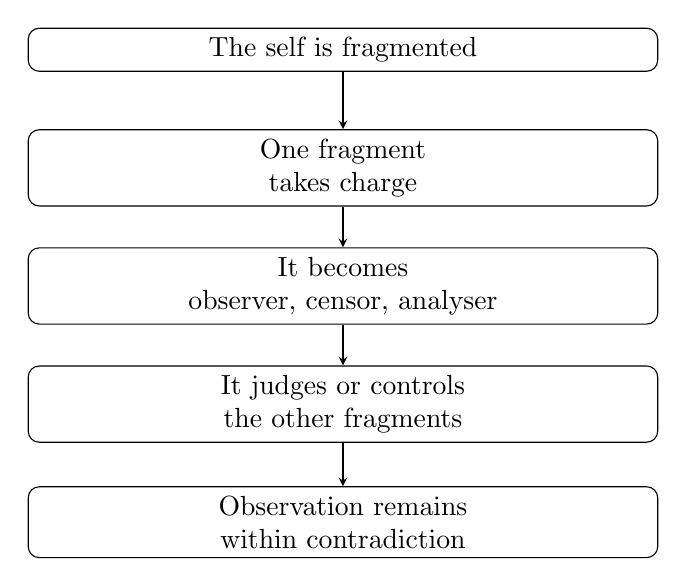
\begin{tikzpicture}[>=stealth]
\node[draw, rounded corners, text width=.64\linewidth, align=center] (f1) at (0,0) {The self is fragmented};
\node[draw, rounded corners, text width=.64\linewidth, align=center] (f2) at (0,-1.5) {One fragment\\takes charge};
\node[draw, rounded corners, text width=.64\linewidth, align=center] (f3) at (0,-3.0) {It becomes\\observer, censor, analyser};
\node[draw, rounded corners, text width=.64\linewidth, align=center] (f4) at (0,-4.5) {It judges or controls\\the other fragments};
\node[draw, rounded corners, text width=.64\linewidth, align=center] (f5) at (0,-6.0) {Observation remains\\within contradiction};
\draw[->] (f1) -- (f2);
\draw[->] (f2) -- (f3);
\draw[->] (f3) -- (f4);
\draw[->] (f4) -- (f5);
\end{tikzpicture}
\end{figure}

\begin{proposition}
If the observer is itself a fragment, observation by that observer cannot end fragmentation.
\end{proposition}

\begin{proof}
The observer is one part of the divided field. When that part claims authority over the other parts, division has not ended; it has taken the form of control. The observer may condemn, justify, approve, store up, or attempt to alter what it sees, but those movements are themselves fragmentary. Therefore such observation remains within contradiction.
\end{proof}

This proposition is not an imported psychological doctrine. It is simply the lecture's argument written in a compact form. As long as one fragment watches the rest from a position of authority, the structure of division continues.

\section{The Observer, The Image, And Violence}

Krishnamurti next asks whether we observe through an image. We look at a tree through knowledge of the tree. We look at wife, husband, friend, opponent, Catholic, Protestant, communist, or bourgeois through images accumulated over years, or perhaps only days. The image stands between observer and observed.

The sequence is
\begin{equation}
\text{knowledge}
\;\longrightarrow\;
\text{image}
\;\longrightarrow\;
\text{observer}
\;\longrightarrow\;
\text{separation}.
\end{equation}
The important step is the third one: the image becomes the observer. The observer is not a pure witness outside conditioning. It is built from memory, judgement, naming, hurt, flattery, insult, belief, fear, and desire.

The lecture then tests the matter against violence. This is the right test because violence is not merely an idea. Suppose I am violent: angry, jealous, brutal, ambitious, always measuring myself against another. If I then say, ``I must get rid of violence,'' who is the ``I'' that says this? Is it separate from violence, or is it part of the same movement?

\subsection{Question \& Answer}

\paragraph{Question.}
Is the observer different from violence?

\paragraph{Answer.}
Krishnamurti's answer is that this separation is one of the tricks of thought. The observer who condemns violence, justifies violence, or tries to escape violence is not outside violence. In this precise sense,
\begin{equation}
\text{observer} = \text{observed}.
\end{equation}
This is not a mathematical identity and not a general metaphysical slogan. It means that the observer looking at violence is part of the same movement as violence.

The contrary assumption gives the old structure:
\begin{equation}
\text{observer} \neq \text{observed}
\quad\Longrightarrow\quad
\text{division}
\quad\Longrightarrow\quad
\text{conflict}.
\end{equation}
So long as there is division between observer and observed, conflict continues. When the observer sees that it is not separate from what is observed, the machinery of condemnation, justification, and escape no longer operates in the same way.

\begin{figure}
\centering
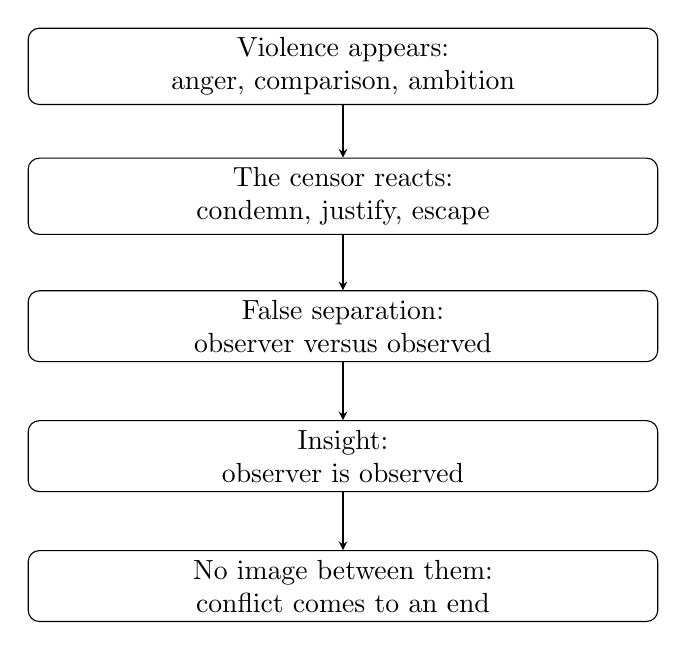
\begin{tikzpicture}[>=stealth]
\node[draw, rounded corners, text width=.64\linewidth, align=center] (a) at (0,0) {Violence appears:\\anger, comparison, ambition};
\node[draw, rounded corners, text width=.64\linewidth, align=center] (b) at (0,-1.65) {The censor reacts:\\condemn, justify, escape};
\node[draw, rounded corners, text width=.64\linewidth, align=center] (c) at (0,-3.30) {False separation:\\observer versus observed};
\node[draw, rounded corners, text width=.64\linewidth, align=center] (d) at (0,-4.95) {Insight:\\observer is observed};
\node[draw, rounded corners, text width=.64\linewidth, align=center] (e) at (0,-6.60) {No image between them:\\conflict comes to an end};
\draw[->] (a) -- (b);
\draw[->] (b) -- (c);
\draw[->] (c) -- (d);
\draw[->] (d) -- (e);
\end{tikzpicture}
\end{figure}

The transcript is damaged in a short stretch near this point, but the surrounding movement is coherent. Identification is another form of separation: the mind separates itself as censor and then tries to identify with what it calls noble, beautiful, or desirable. Where there is no image between observer and observed, Krishnamurti says, conflict comes to an end. He calls this real meditation, not a trick; in this chapter we keep that phrase tied to this specific structure of observation.

\section{Learning Without Accumulation}

The final difficulty is subtler and easy to miss. One observes oneself and learns something. Then, the next minute, one may look again through what one has just learned. If that happens, has learning continued, or has the previous observation become accumulated knowledge?

Let $I_n$ denote the image or accumulated residue through which one looks at moment $n$. In the ordinary movement of accumulation,
\begin{equation}
I_{n+1}
=
I_n
\cup
\{\text{insult},\text{flattery},\text{judgement},\text{previous observation}\}.
\end{equation}
Then the next act of seeing is filtered through the updated residue:
\begin{equation}
\text{seeing}_{n+1}
=
\text{observation through } I_{n+1}.
\end{equation}
This notation is a warning. It shows how yesterday's observation can become today's observer. The accumulation itself becomes the censor, the conditioned entity, the image through which the next perception is formed.

\paragraph{Worked example: flattery and insult.}
Suppose someone flatters us or insults us. If the words are accumulated, the update is
\begin{align}
I_{n+1}
&= I_n \cup \{\text{flattery}\}
&&\Longrightarrow\quad \text{the speaker becomes friend},\\
I_{n+1}
&= I_n \cup \{\text{insult}\}
&&\Longrightarrow\quad \text{the speaker becomes enemy}.
\end{align}
In either case, listening has created an image. The image separates. From then on one no longer listens directly; one listens through the stored picture.

The alternative is not suppression and not a cultivated method. It is to listen without accumulating the insult or the flattery. The same structure applies at the moment of anger. If one is not aware then, the image has already begun to form; the censor has already taken its position.

\begin{definition}
Observation without accumulation means looking or listening without carrying forward insult, flattery, naming, previous conclusion, or self-image as the basis for the next perception.
\end{definition}

Krishnamurti closes this movement with simple acts of observation: cloud, hills, light on water. To observe without naming is to see how naming, knowledge, and experience can prevent the mind from observing totally. When the mind looks without the observer, he says, the fragments come to an end in oneself. This cannot be taught by another.

\section{Summary}

The lecture begins with the disorder of the world and moves step by step toward the act of observation. Division appears outwardly as nation, religion, profession, ideology, and social conflict; it appears inwardly as contradiction, fear, anger, ambition, comparison, image, and accumulated knowledge. The opening question, ``what is one to do?'', cannot be answered by another fragment.

The inquiry therefore turns from program to whole action, from whole action to right relationship, and from right relationship to self-observation. The speaker is not an authority but a mirror. The world is not merely outside oneself; the world and the self share the same movement of division.

The central question becomes: how do we observe? If one fragment observes the rest, the observer remains part of fragmentation. If we observe through image, knowledge, naming, flattery, insult, or previous experience, the image becomes the observer and separation continues. In the lecture's decisive formulation, the observer is the observed. To see this directly, without turning it into a slogan or method, is the act of learning.